% This work is licensed under the Creative Commons Attribution NonCommercial
% ShareAlike 4.0 International License. To view a copy of the license, visit
% https://creativecommons.org/licenses/by-nc-sa/4.0/

\thispagestyle{empty}~
\clearpage

\thispagestyle{empty}
\color{white}
\newpagecolor{covercolor}
\newgeometry{
  body={118mm,185mm},
  hcentering,
  vcentering,
  headsep=2pc}

\noindent {\sffamily\fontsize{16}{18}\bfseries\selectfont
Programming a toy computer from scratch}

\bigskip

\noindent This book introduces how computer hardware, programming languages and
operating systems work, via a practical example which can be understood down to
the smallest detail. For this it explains how you can assemble and program a
toy computer, in an entirely bottom-up way, without using any existing
programming tool. The end result is a toy, monotasking operating system with a
command line shell, a text editor, a compiler, and a few utilities, in less
than 3300 lines.

\noindent
\begin{tikzpicture}[overlay]
  \node[anchor=north west,inner sep=0] at (0,-0.5cm)
  {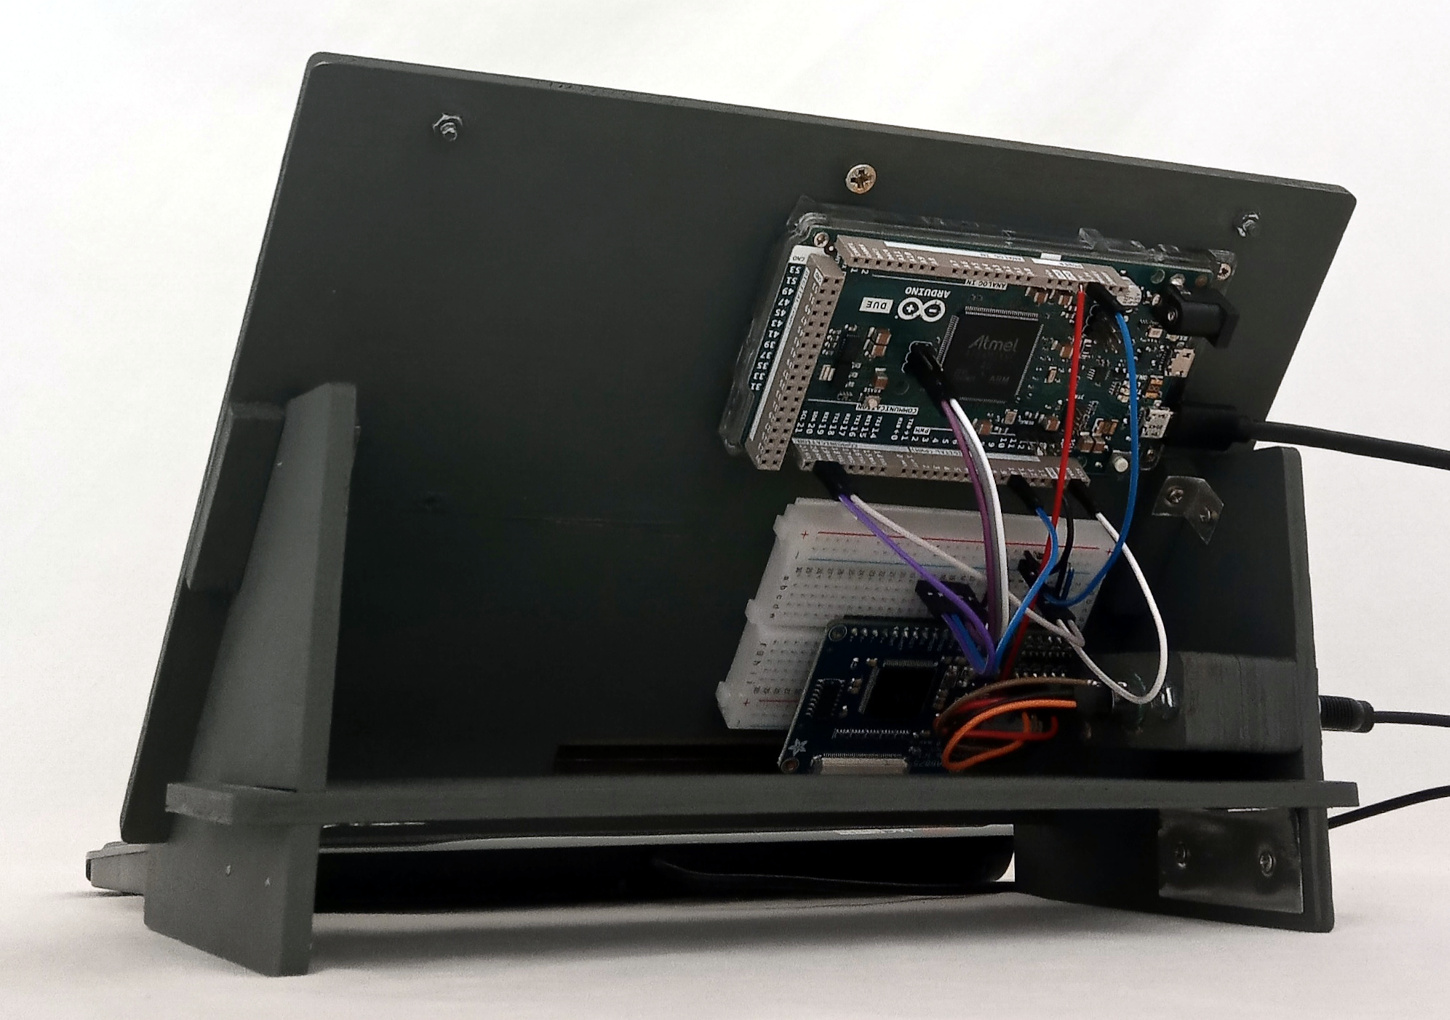
\includegraphics[width=\textwidth]{cover/back}};
\end{tikzpicture}

